% Tento soubor nahraďte vlastním souborem s obsahem práce.
%=========================================================================
% Autoři: Michal Bidlo, Bohuslav Křena, Jaroslav Dytrych, Petr Veigend a Adam Herout 2019

% Pro kompilaci po částech (viz projekt.tex), nutno odkomentovat a upravit
%\documentclass[../projekt.tex]{subfiles}
%\begin{document}

\chapter{Úvod}
Podpis je jednou z~nejstarších metod používanou pro ověření totožnosti, určení autorství či udělení právního souhlasu.
Dodnes se stále používá pro jeho uživatelskou přívětivost a akceptovatelnost zákonem. %?
S technologiemi dnešní doby není problémem tento podpis digitalizovat a používat ho k automatizované autentizaci. %?
V~této práci půjde práve o oklamání automatizované autentizace pomocí replikace vlastnoručního podpisu.
Autentizace spadá pod obor zvaný biometrie, která se zabývá analýzou biologických a behaviorálních charakteristik. 
%Zkoumáním pravosti podpisu a jiných textů se zabývá písmoznalectví neboli grafognózie.
U~podpisu lze pak analyzovat dvě skupiny charakteristik písma, a to statické a dynamické. 
Statické jsou charakteristiky, které lze extrahovat z hotového podpisu.
Oproti tomu dynamické musí být zaznamenávány v průběhu podpisu.

Podpis je v~praxi stále nejpoužívanější způsob autentizace v pravních, komerčních či jiných oblastech. 
Pro autentizaci se zkoumají především dynamické vlastnosti písma, jelikož je mnohem těžší je replikovat a tedy zajišťují větší bezpečnost.
Podaří-li se důvěryhodně vlastnoruční podpis replikovat, bude možné pomocí falzifikátu obejít bezpečnostní zabezpečení. 
To představuje velké bezpečnostní riziko a nutnost upravení dosavadních bezpečnostních metod pro autentizaci. 


%TOLE JE SPIS ABSTRAKT
%Bude třeba sestavit snímací zařízení pro získaní potřebných parametrů podpisu.
%Ze statických parametrů budeme snímat tvar i tloušťku čar a celkový vzhled podpisu. 
%Z dynamických parametrů budeme snímat tlak, sklon a průběh tahů. 
%Získané data je potřeba vhodným způsobem zpracovat a provést potřebné výpočty. 
%Upravená data je poté potřeba převést do instrukcí pro mechanickou paži, která je použita k replikaci podpisu. 
%Výsledný podpis bude porovnáván s vlastnoručním podpisem. Cílem je co nejvíce se přiblížit vlastnoručnímu podpisu.

%\section{Představení tématu}
%\section{Cíle práce}

%\section{Struktura práce}

\chapter{Teoretické základy}
Pro plné pochopení problematiky je potřeba představit základy z~několika odvětví. 
V~této části budou shrnuty všechny potřebné informace. 

\section{Pojmy}\label{sec:pojmy}
\begin{itemize}
  \item \textbf{Biometrie} --- automatizované rozpoznávání osob na základě jejich charakteristických biologických a behaviorálních rysů. % parafráze biometrie (str. 13) / Biometric identification - parafráze (str 3)
  \item \textbf{Biologické autentizační metody} --- zkoumají biologické charakteristiky člověka, s~jimiž se narodí. Tyto charakteristiky má každý člověk unikátní a jsou neměnitelné. Patří mezi ně například otisky prstů, skeny sítnice či duhovky.  
  \item \textbf{Behaviorální autentizační metody} --- porovnávají behaviorální charakteristiky související s~chováním člověka. Lze například porovnávat, jakým způsobem jedinec mluví nebo jak pohybuje očima.
  \item \textbf{Statické parametry písma} --- jde o~parametry, které nezahrnují informace o~procesu psaní podpisu. Patří mezi ně například tvar a vzhled písma, umístění podpisu na stránce nebo také tloušťka čar.
  \item \textbf{Dynamické parametry písma} --- tyto parametry se vztahují k~samotnému průběhu psaní podpisu. Například rychlost psaní, akcelerace, tlak nebo průběh tahů.
\end{itemize}

Dále je potřeba si ujasnit tyto tři pojmy:
\begin{itemize}
  \item \textbf{Verifikace} --- potvrzení totožnosti jedince porovnáním poskytnutého vzoru s referenčními vzorem dané osoby uloženého v databázi, % |
  za kterou se vydává. Probíhá tedy principem one-to-one.                                                                                     % |
  \item \textbf{Identifikace} --- určení identity předem neznámého jedince.                                                                       % |
  Jde tedy o přikládání poskytnutého vzoru ke všem vzorům v databázi, tedy princip one-to-many.                                                % |
  \item \textbf{Autentizace} --- je proces, vyskytující se především u přistupových systému.                                                      % |
  Může se u ni jednat při verifikaci i identifikaci.                                                                                            % V
  Výsledkem bývá získání nějakého statusu, například získání určitých oprávnění.                                                       % Biometrické technologie (str. 4-5) https://www.fbi.vsb.cz/export/sites/fbi/060/.content/galerie-souboru/studijni-materialy/BiometrickeTechnologie.pdf
\end{itemize}


\section{Definice podpisu a jeho charakteristiky}
Definice podpisu je z~pohledu zákona poněkud problematická. 
Podpis jako takový není v~zákoně nijak přímo definován. 
Obecně je ale bráno za podpis vlastnoruční uvedení jména a příjmení, nebo jiného jedinečného a nezaměnitelného označení. % citace? https://www.fulsoft.cz/33/komentar-zakona-89-2012-sb-obcansky-zakonik-561-uniqueidmRRWSbk196FNf8-jVUh4EtuvCojfP1Dmx8t50X_QR_yU_dtwjPItMA/

Dynamické vlastnosti poskytují více informací a umožňují lépe identifikovat neoprávněného uživatele, pokoušejícího se podpis falzifikovat.    % V
K zaznamenání těchto dynamických vlastností je avšak zapotřebí tablet a speciální aktivní pero, které při psaní ukládá relevantní parametry.  % parafráze Citace Biometrie (str 233)

Podpis patří z části ke statickým a z části k dynamickým biometrickým vlastnostem.
Pokud se uchovává pouze výsledek psaní podpisu, lze z něj extrahovat pouze statické parametry.
Pro snímání dynamických parametrů je nutné snímat podpis v průběhu jeho psaní.
Těchto parametrů je mnoho, ale pro zjednodušení se jich používá jen omezené množství.

\section{Biometrická autentizace}
Biometrie je jedním ze tří hlavních kategorií autentizace.
autentizova se můžeme pomocí toho:

\begin{itemize}
  \item co vlastníme --- identifikační doklady, karty, čipy\ldots   % ? | 
  \item co známe --- přihlašovací jména, hesla\ldots                % ? |
  \item čím fyzicky jsme --- otisky prstu, tvář, oči, podpis\ldots  % ? V
\end{itemize}                                                   % parafráze Biometrie a identita člověka (str 89) 
Biometrie spadá do třetí kategorie, tedy čím fyzicky jsme. 

Biometrická autentizace probíhá na základě biologických a behaviorálních charakteristik člověka\ref{sec:pojmy}. 
Obě tyto skupiny znaků jsou pro každého člověka unikátní a nezaměnitelné. To je důvodem, proč je lze využít k~autentizaci.
Existuje spousta biometrických metod pro autentizaci, kupříkladu otisk prstu, rozpoznání obličeje, sken duhovky či sítnice, nebo dokonce pomocí používání myši. 
Každá tato metoda má své výhody a nevýhody, zejména se hodnotí přesnost, cena, komfort používání, stálost a velikost vzorku. % ?
Tato práce se zaměřuje na autentizaci pomocí podpisu.

Biometrický systém je v informačních technologiích postup pro rozpoznávání vzorů lidských vlastností.       % |
Existuje spoustu různých cest, kterými lze biometrické systémy napadnout.                                   % |
V~rámci této práce se zaměříme na seznzor, jenž je první komponentu biometrického systému (obrázek níže).   % V
Tomuto senzoru budeme předkládat falešné biometriky, tedy v~našem případě falešného podpisu.                % parafráze Biometrie (str 78)

\begin{figure}[h]\label{fig:my-pdf}
  \centering
  
\includegraphics[width=0.5\textwidth]{obrazky-figures/placeholder.pdf}
  \caption{Biometrický systém --- Biometrie (str. 78)}
\end{figure}

\newpage

\section{Parametry podpisu}
V~rámci této práce budou snímány následující parametry:
\begin{itemize}
  \item \textbf{Celkový vzhled podpisu}
  \item \textbf{Pohyb pera} ze kterého bude vypočítán celkový průběh podpisu, především pak pozice pera a rychlost psaní čar. %při psaní pomocí akcelerometru zabudovaném v MPU-6050 
  \item \textbf{Sklon pera} %pomocí gyroskopu, který je také součástí MPU-6050.}
  \item \textbf{Tlak} %pomocí čtveřice tlakových senzorů Interlink Electronics FSR® 400.}
\end{itemize}
Kombinací těchto nasnímaných parametrů by bylo možné dostatečně věrohodně napodobit původní vlastnoruční podpis. 

\section{Rozpoznávání falzifikátů}
Rozpoznání falzifikátu probíhá u statického a dynamického podpisu odlišně, následující text se bude týkat postupu, který sdílejí.

Falzifikáty jsou vyhodnoceny na základě porovnávání uloženého vzorku v~databázi s~podpisem, kterým se daný člověk pokouší autentizovat.
Výsledkem takového porovnávání je určité procento shody parametrů.
Referenční podpis je zprůměrován z~několika vzorků, aby došlo k~potlačení náhodných jevů. %  citace? zav_prace 17183 2.3
Tyto vzorky jsou poskytnuté danou osobou při registraci do systému.

\begin{figure}[h]\label{fig:my-pdf}
  \centering
  
\includegraphics[width=0.5\textwidth]{obrazky-figures/placeholder.pdf}
  \caption{Průběh autentizace}
\end{figure}

Obě tyto skupiny charakteristik jsou ovlivňovány jak fyzickým, tak i psychologickým stavem člověka v~době podpisu.
To znamená, že ani též osobě se nepovede dvakrát úplně totožný podpis.
Pokud jsou podpisy naprosto stejné, nejspíše půjde právě o padělek.

Porovnávací algoritmus extrahuje důležité parametry podpisu, které poté porovnává s~referenčním vzorem. 
Následně je vypočteno celkové procento shody podpisů a na jeho základě je autentizace úspěšná či nikoli.
Je přitom důležité, aby algoritmus měl určenou správnou procentuální hodnotu shody. 

Pokud by bylo procento shody špatně zvoleno, došlo by k jednomu ze dvou problémů:
\begin{itemize}
  \item \textbf{míra falešných odmítnutí (FRR)} --- neúspěšné autentizace, které by měly být úspěšné.
  \item \textbf{míra falešných akceptací (FAR)} --- úspěšné autentizace, které by měly být neúspěšné.
\end{itemize}

Výše zmíněné procento shody nazýváme rovnoměrná míra chybovosti (EER), pokud je nastavena právě v bodě protnutí těchto dvou křivek (viz~\ref{fig:FAR_FRR}).

\begin{figure}[h]\label{fig:FAR_FRR}
  \centering
  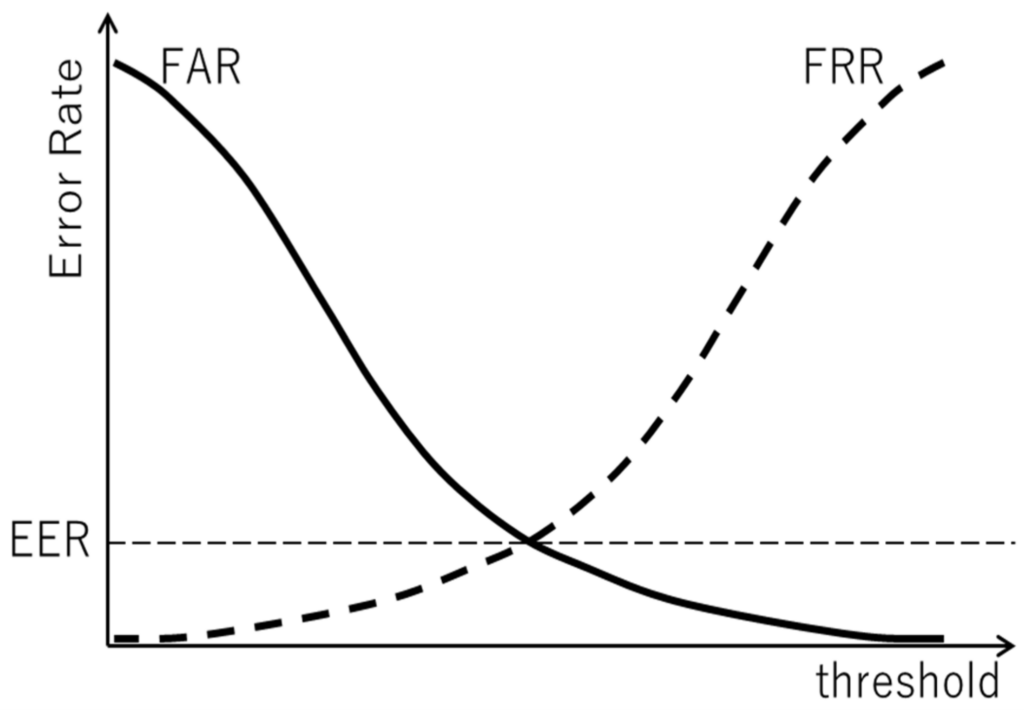
\includegraphics[width=0.5\textwidth]{obrazky-figures/FAR_FRR.png}
  \caption{Rovnoměrná míra chybovosti (EER), míra falešných odmítnutí (FRR) a míra falešných akceptací (FAR)} % https://www.cursorinsight.com/post/943/what-you-need-to-know-about-frr-and-far
\end{figure}

\newpage

\section{Off-line systémy pro verifikaci}
Off-line systémy pro verifikaci se rozumí systémy, které ověřují totožnost na základě statického podpisu, tedy psaného na papír.  % |
Obraz podpisu je naskenován či nasnímán kamerou a tím je získán digitální obraz podpisu.                                          % |
Tento obraz je následně porovnáván v databázi s referenčním podpisem.                                                             % |
Tato metoda je avšak nepoužitelná, co se týče automatizovaného zpracování.                                                        % V
Navíc v dnešní moderní době, při existenci skenovacích a kopírovacích zařízení, je statický podpis náchylný na falzifikaci.       % Parafráze Biografie a identita člověka (str 440)

Verifikace probíhá ve třech fázích --- předzpracování, extrakce biometrických charakteristik a vyhodnocování. % |
V předzpracování projde naskenovaný obraz podpisu prahováním, vyhlazováním, normalizaci a zjednodušování.     % |
Následně jsou extrahovány biometrické charakteristiky podpisu,                                                % |
napřiklad hustota vodorovných a svislých čar, nebo vektory ohraničené oblasti.                                % |
Vyhodnocování je založeno na extrahovaných charakteristikách a jejich vektorech,                              % V
může být provedeno porovnáním významových bodů, klasifikátorem sousedů nebo neuronovou sítí.                  % Parafráze Biometrie a identita člověka (strana 441 442 443) - nebo https://theses.cz/id/odwy80/BP_Vchov.pdf

\begin{figure}[h]
  \centering
  \begin{minipage}{0.3\textwidth}\label{fig:first-image}
    \centering
    
\includegraphics[width=\textwidth]{obrazky-figures/placeholder.pdf}
    \caption{Předzpracovaný podpis.}
  \end{minipage}\hfill
  \begin{minipage}{0.3\textwidth}\label{fig:second-image}
    \centering
    
\includegraphics[width=\textwidth]{obrazky-figures/placeholder.pdf}
    \caption{Extrahované parametry.}
  \end{minipage}\hfill
  \begin{minipage}{0.3\textwidth}\label{fig:third-image}
    \centering
    
\includegraphics[width=\textwidth]{obrazky-figures/placeholder.pdf}
    \caption{Vyhodnocování.}
  \end{minipage}
\end{figure}

\section{On-line systémy pro verifikaci} 
On-line systémy narozdíl od off-line neporovnávají pouze výsledek podpisu, ale i data o jeho průběhu. % |
Důležité zde jsou parametry jako změny rychlosti, tlaku a celkovém průběhu psaní podpisu.             % |
K nasnímání těchto parametrů je potřeba tablet a speciální pero, které takové snímání umožní.         % |
Narozdíl od statických parametrů, které lze snáze odpozorovat a napodobit,                            % |
nebo pomocí technologií jinak replikovat, je dynamické parametry nemožné zfalšovat člověkem.          % V
Falzifikát lze vytvořit pomocí stroje, je k tomu ale potřeba nasnímat pohyb ruky podepisujícího.      % parafráze Biometric verification (str. 170)

\begin{figure}[h]
  \centering
  \begin{minipage}{0.45\textwidth}\label{fig:first-image}
      \centering
      
\includegraphics[width=\textwidth]{obrazky-figures/placeholder.pdf}
      \caption{Vzhled dynamického podpisu.}
  \end{minipage}\hfill
  \begin{minipage}{0.45\textwidth}\label{fig:second-image}
      \centering
      
\includegraphics[width=\textwidth]{obrazky-figures/placeholder.pdf}
      \caption{Graf dynamických parametrů podpisu v~čase.}
  \end{minipage}
\end{figure}

\section{Biometrické normy identifikace pomocí podpisu}

Vytvoření norem mělo velký pozitivní dopad na rozšíření biometrických systémů.                                                % |
Jde napřiklad o normy určující, jakým způsobem mají být biometrická data ukládána či jakým způsobem dochází k jejich vyměně.  % | 
Tyto normy přispěly k větší interoperabilitě jednotlivých komponent biometrických systémů.                                    % V
To znamená, že lze jeden komponent vyměnit za stejný od jiného výrobce a neměl by být problém s kompatibilitou.               % parafraze Biologie str. 61

Normy obecně přinášejí několik zásadních výhod:
\begin{itemize}
  \item Interoperabilita: Umožňují výměnu dat mezi různými systémy a zařízeními bez ztráty integrity nebo kompatibility.
  \item Bezpečnost: Standardizované formáty zajišťují ochranu citlivých dat a minimalizují riziko neoprávněného přístupu.
  \item Spolehlivost: Poskytují jednotné metody pro ukládání a zpracování dat, což zvyšuje přesnost a důvěryhodnost biometrických systémů.
  \item Právní jistota: Splnění norem často znamená, že technologie odpovídá požadavkům právních a regulačních předpisů.
\end{itemize}

Autentizace vlastnoručním podpisem spadá pod několik norem, zaměřující se například na zachycení a uložení dat o podpisu, nebo způsob, jakým se tato data budou vyměňovat. 
Mezi nejdůležitější patří:

\subsection*{ISO/IEC Normy}
\begin{itemize}
  \item \textbf{ISO/IEC 19794-1:2011 (Framework)}: 
  Definuje obecný formát pro ukládání a používání biometrických dat, konvenci pojmenování datových struktur a podobně. % parafraze ISO/IEC 19794-1:2011 str. 1

  \item \textbf{ISO/IEC 30107-3:2017 (Biometric Presentation Attack Detection)}: 
  Tato norma se zabývá technikami pro automatickou detekci prezentačních útoků. % parafraze ISO/IEC 30107-3:2017 str. 1

  \item \textbf{ISO/IEC 19794-7:2021 (Signature/sign time series data)}:
  Specifikuje formát pro ukládání a výměnu dat pro dynamické podpisy. 
  Formát lze vidět na obrázku \ref{fig:norms_table}. 
  Verze 2021 je novější verze té stejné normy z roku 2007. % parafraze ISO/IEC 19794-7:2021 str. 1
\end{itemize}

\begin{figure}[h]\label{fig:norms_table}
  \centering
  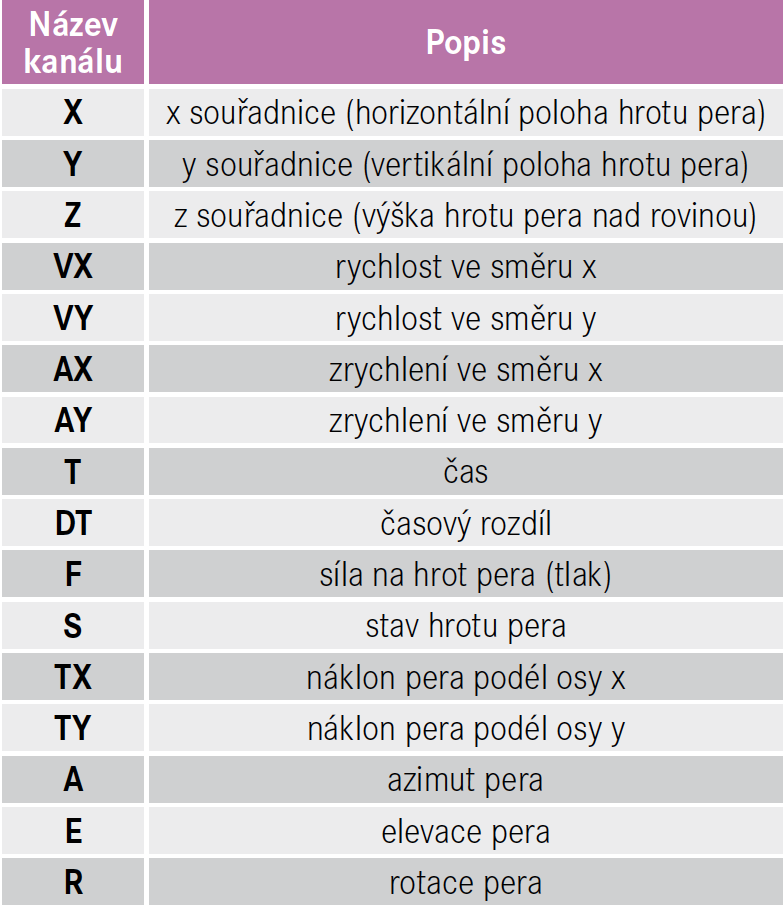
\includegraphics[width=0.5\textwidth]{obrazky-figures/normy.png}
  \caption{Struktura zaznamenávaných dat daná normou ISO/IEC 19794-7:2021.} % https://dsm.tate.cz/cs/2021/dsm-3-2021/vlastnorucni-podpis-a-informacni-systemy-necekane-spojeni?utm_source=chatgpt.com
\end{figure}

\subsection*{ANSI/INCITS Normy}
\begin{itemize}
  \item \textbf{ANSI/INCITS 395-2005 (Signature/Sign Data)}  
  Definuje obecný formát pro výměnu dat digitalizovaného podpisu. Díky své obecnosti lze použít v široké škále aplikací. % parafraze ANSI/INCITS 395-2005 str. 1
  
  \item \textbf{ANSI/INCITS 398-2005 (Common Biometric Exchange Format Framework)}  
  Definuje soubor datových prvků potřebných k zajištění univerzální podpory různých biometrických technologií a stanovuje požadavky pro zajištění vzájemné kompatibility. % parafraze biometrie str. 69
\end{itemize}

Existuje spousta dalších norem týkajících se jak biometrie, jiných biometrických metod či přímo digitálního podpisu.                % |
Kromě již zmíněných organizací existují další organizace, zabývající se normami pro biometrii.                                      % V
Například NIST, působící na poli biometrických databází, TCSEC, Common Criteria, obojí zabývající se biometrií v rámci bezpečnosti. % Biometrie str. 68

Normy v oblasti biometrického podpisu tvoří klíčový základ pro spolehlivé a bezpečné využití těchto technologií v praxi.


\chapter{Analýza současných řešení}

V současné době nabývají na významu biometrické systémy založené na využití vlastnoručních podpisů. 
Tyto systémy se úspěšně používají například v oblasti bankovnictví, elektronického obchodu, správy elektronických dokumentů a dalších oblastech, kde je potřeba provést autentizaci jedince. 
Existují dva přístupy k autentizaci uživatelů.
První je založena na statických parametrech („off-line“) --- zahrnuje rozpoznání podpisu osoby na základě analýzy jeho vzhledu.
Druhý je pak založen na dynamických parametrech („on-line“) --- zahrnuje čtení a rozpoznávání informací o dynamice psaní vlastnoručního podpisu. % parafraze  E. S. Anisimova and I. V. Anikin, "Finding a Rational Set of Features for Handwritten Signature Recognition," 2020 Dynamics of Systems, Mechanisms and Machines (Dynamics), Omsk, Russia, 2020, pp. 1-6, doi: 10.1109/Dynamics50954.2020.9306154.

Ne všechny údaje (viz \ref{fig:norms_table}) jsou přítomny u každého podpisového řešení a vedle dat získaných přímo z digitalizačního zařízení, např. data o poloze hrotu pera, jde také o data dopočítaná, třeba údaje o rychlosti nebo zrychlení. %!
V praxi se nejčastěji využívají data z kanálů X, Y, T a F. To znamená, že systém v každém momentu vzorkování zaznamená polohu hrotu pera v rovině (X, Y), čas záznamu (T) a sílu působící na hrot pera (F). %! https://dsm.tate.cz/cs/2021/dsm-3-2021/vlastnorucni-podpis-a-informacni-systemy-necekane-spojeni?utm_source=chatgpt.com

\subsection*{Záznamová zařízení}
K zaznamenávání dynamického podpisu lze použít několik typů zařízení.

%TODO
%Technologie automatického ověřování podpisu se v současnosti řadí mezi klíčové oblasti výzkumu.                                                         % |
%Především díky své důležitosti ve vědeckém a komerčním kontextu.                                                                                        % |
%S rychlým rozvojem internetu a rostoucími požadavky na bezpečnost v digitální společnosti se tato technologie stává stále relevantnější.                % |
%Poskytuje efektivní a důvěryhodnou metodu ověřování identity, která je v současnosti široce akceptována jak z právního, tak ze společenského hlediska.  % V
%To ji činí zásadním nástrojem pro současné technologické aplikace.                                                                                      % Impedovo

\section{Současná řešení v~oblasti biometrie}
%Nedávné mezinárodní soutěže využívající standardní databáze a testovací protokoly přinesly zajímavé výsledky.   % |
%Ukázalo se, že systémy pro ověřování podpisů dosahují vysoké přesnosti.                                         % V
%Tato úroveň přesnosti je srovnatelná s jinými pokročilými biometrickými technologiemi.                          % C. Vielhauer, “A behavioural biometrics,” Public Service Rev.: Eur.Union, vol. 20, no. 9, pp. 113–115, 2005.

%Na rozdíl od fyziologické biometrie je vlastnoruční podpis aktivní metodou.                                                   % |
%Ta vyžaduje, aby uživatel provedl konkrétní akci podpisu.                                                                     % V
%Automatické ověřování podpisu je tedy obzvláště užitečné v aplikacích, kde je nutná autentizace jak uživatele, tak transakce. % Plamondon and S. N. Srihari, “On-line and offline handwriting recog-nition: A comprehensive survey,” IEEE Trans. Pattern Anal. Mach.Intell., vol. 22, no. 1, pp. 63–84, Jan. 2000

%Systémy pro verifikaci podpisu se obvykle skládají z hardwarových a softwarových komponent.%!
%Ty spolupracují při ověřování autenticity podpisu. %!
%Zařízení pro sběr podpisu mohou zahrnovat dotykové obrazovky, grafické tablety nebo speciální senzory, zaznamenávající různé parametry podpisu.%!
%Takovými parametry jako je tlak, rychlost a trajektorie pohybu ruky. % \cite{novak2022}, \cite{kriz2019}.%!

\section{Systém, zařízení a kde se využívají, a jak jsou důvěryhodné}
%Tyto systémy jsou široce využívány v bankovnictví, právních službách, elektronických platbách a dalších oblastech, ve kterých je nutné ověřit identitu uživatele a zajistit integritu transakce.%!
%Důvěryhodnost těchto systémů závisí na několika faktorech, včetně kvality zařízení pro sběr dat, algoritmů pro analýzu podpisu a úrovně šifrování použité při přenosu dat. %!
%Vysoká úroveň přesnosti a spolehlivosti je kladně ovlivněna používáním pokročilých metod strojového učení a biometrických analýz, které zajišťují, že systém dokáže rozlišit mezi autentickým podpisem a padělaným. %!
%Přesto i u těchto systémů existují určité výzvy, jako je možnost podvodů prostřednictvím simulace podpisu nebo použití záznamů starých podpisů. %!
%Z tohoto důvodu je důležité kombinovat různé metody autentizace pro dosažení co nejvyšší úrovně bezpečnosti. % \cite{vodicka2021}, \cite{hanzelka2020}.%!

\section{Hodnocení výhod a nevýhod existujících řešení}
%Existující řešení pro verifikaci podpisu nabízejí několik výhod a nevýhod v závislosti na použité technologii a aplikacích. %!
%Mezi hlavní výhody patří vysoká úroveň bezpečnosti, kterou poskytují biometrické metody.%!
%Analýza dynamiky podpisu, jako je měření rychlosti, tlaku a trajektorie pohybu ruky, zvyšuje spolehlivost ověření podpisu a umožňuje detekci padělaných podpisů, což je klíčové pro oblasti, jako je bankovnictví a právní služby. % \cite{Jain2004}, \cite{Kumar2016} %!
%Systémy pro verifikaci podpisu mohou být rovněž snadno implementovány v digitálních prostředích, což usnadňuje autentizaci uživatelů při online transakcích a zajišťuje integritu dokumentů.%!

%Na druhé straně existují i nevýhody, které je třeba zvážit při implementaci těchto systémů. %!
%Jedním z hlavních problémů je vysoká cena potřebného hardwaru a softwaru, což může být pro některé organizace překážkou. %!
%Další výzvou je náchylnost biometrických systémů k podvodům, jako je použití padělaných podpisů nebo záznamů starých podpisů, což může ohrozit bezpečnost. % \cite{Kose2017} %!
%Kromě toho přesnost systémů pro verifikaci podpisu může být ovlivněna faktory, jako jsou změny v rukopisných schopnostech uživatele, což může vést k falešným odmítnutím nebo akceptacím podpisu. %\cite{Rathgeb2016}. %!
%Tyto faktory ukazují, že biometrické systémy nejsou bez rizika a měly by být kombinovány s dalšími metodami autentizace pro zajištění maximální bezpečnosti.%!

%Závěrem lze říci, že existující řešení pro verifikaci podpisu nabízejí vysokou úroveň bezpečnosti a efektivity, ale také čelí výzvám, které vyžadují pečlivé zvážení při jejich implementaci a použití.%!
%TODO

\section{Výběr senzorů a technologií}
Výběr senzorů pro nasnímání dynamických parametrů byl složitý vzhledem k rozměru pera a omezenému rozpočtu. % |
Dalším parametrem, který hrál roli při rozhodování, byla přesnost jednotlivých komponent.                   % V
Bylo důležité brát v potaz i to, zda jsou všechny komponenty kompatibilní s použitým mikrořadičem.          % vlatní kec

\subsection*{ESP32}
Mikrořaďič ESP32 je jedním z nejrozšířenějších mikrořadičů používaných ve světě.                            % |
V tomto projektu je osazen na vývojové desce ESP32 DevKitC od firmy Espressif.                              % V
Ta je jednou z nejpopulárnějších vývojových desek založených na mikrořadiči ESP32.                          % The Official ESP32 book (str. 35)
Vývojová deska ESP32 DevKitC zde slouží jako mozek celého snímání.                                          % |
Jsou k ní připojené všechny ostatní komponenty, které právě mikrořadiči odesílají nasnímaná data.           % V
ESP32 poté tyto data zpracovává a odesílá je do počítače, ke kterému je připojen  pomocí USB kabelu.        % vlastní kec

\subsection*{MPU-6050 (akcelerometr a gyroskop)}
MPU-60X0 je první integrované zařízení na světě pro sledování pohybu v šesti osách pomocí           % |
kombinace tříosého gyroskopu, tříosého akcelerometru a digitálního procesoru pohybu.                % V
Je široce využívaný v mnoha odvětvích, kde je potřeba schopnosti přesně sledovat pohyby uživatele.  % https://invensense.tdk.com/wp-content/uploads/2015/02/MPU-6000-Datasheet1.pdf

Zde slouží ke stejnému účelu, a to snímaní dat pohybu pera při podpisu.                             % |
Jak bylo zmíněno v kapitole XY, tyto data jsou potřebná pro extrakci dynamických parametrů podpisu. % V
Snímaná data jsou odesílána v reálném čase mikrořadiči ESP32.                                       % vlastní kec

\subsection*{Tlakový senzor Interlink Electronics FSR® 400}
Model FSR 400 je jednozónový tlakový senzor, tedy má pouze jednu aktivní měřící plochu.                       % |
Rezistory FSR jsou dvouvodičová zařízení a používají robustní polymerové tlustovrstvé snímače.                % |
Ty s rostoucím tlakem na snímač snižují odpor, lze tedy pomocí protékajícího proudu vypočítat sílu stlačení.  % V
Minimální aktivační síla je 0,1 N a maximální citlivost je do 20 N.                                           % https://www.interlinkelectronics.com/fsr-400


\chapter{Návrh snímacího pera}
Pro nasnímání podpisu bylo potřeba sestrojit speciální pero.                                        % |
Toto pero v průběhu podepisování zaznamenává polohu pera ve trojrozměrném prostoru,                 % |
jeho náklon a tlak, který je perem vyvíjen na papír.                                                % |
V rámci této práce není důležité, aby tyto snímače a celkový systém byl skrytý před uživatelem.     % |
Šlo tedy pouze o vymodelování pera, do kterého bude možné jednotlivé komponenty uložit.             % |
Komponenty bylo nutné připevnit pevně, aby bylo možné snímat přesné a korektní informace o podpisu. % |
Pokud by jednotlivé komponenty nebyly správně upevněny,                                             % V
mělo by to negativní vliv na nasbírané informace a tedy na celou replikaci podpisu.                 % vlastní kec
 
\section{Schéma a popis návrhu}
Návrh snámacího pera (obrázek) je navrhnut tak, aby fungoval jako normální pero, 
přičemž bylo zárověň možné snímat jeho pohyb a další dynamické vlastnosti.
Toho je dosáhnuto pomocí připevnění mikrořadiče a ostatních komponent přímo na pero.

\begin{figure}[h]\label{fig:pero}
  \centering
  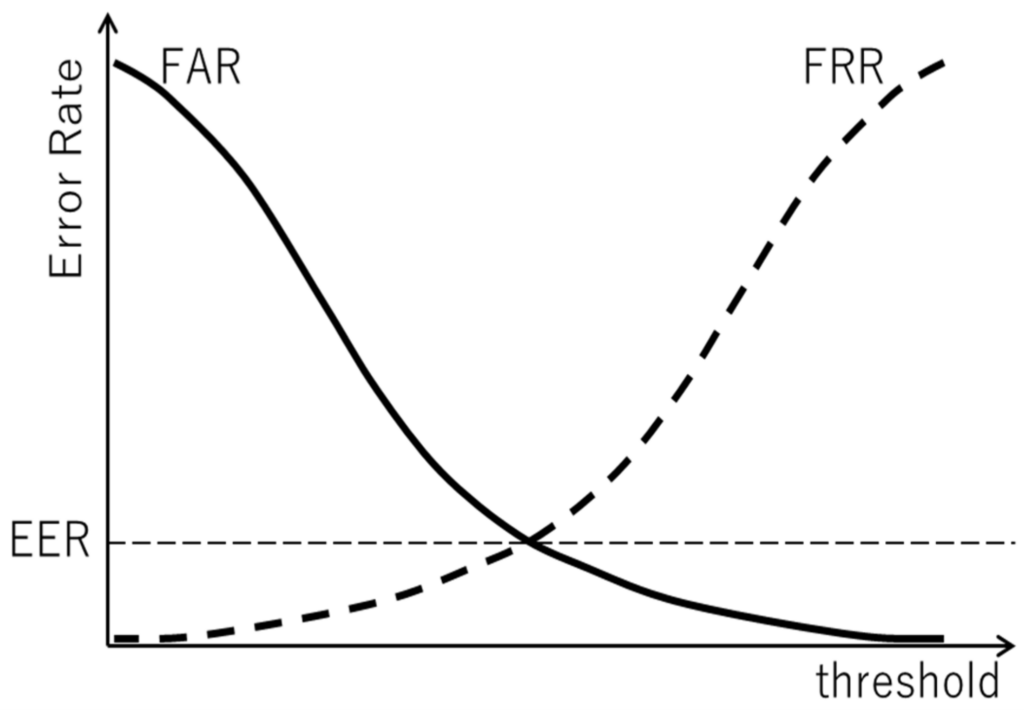
\includegraphics[width=0.5\textwidth]{obrazky-figures/FAR_FRR.png}
  \caption{Pero} 
\end{figure}

Do tohoto pera je možné uložit jak samotný mikrořadič ESP32 (viz 1), akcelerometr a gyroskop na čipu MPU-6050 (viz 2) tak i tlakové snímače FSR-400.
Tyto tlakové snímače jsou rozmístěny tak, aby se podařilo zachytit co nejvíce informací o tlaku.
Jeden je tedy umístěn nad samotnou náplní propisky, nejvíce využit při psaní kolmo (viz 3).
Tři další jsou poté rozmístěny u hrotu propisky pro přesnější snímání v případě, že je pero nakloněno (viz 4). 


\section{Možnosti replikace podpisu}
Replikovat podpis, jinak také vytvořit falzifikát, lze několika způsoby.

\begin{itemize}
  \item \textbf{Vlastnoruční replikace} --- 
  Napodobení samotného statického podpisu je obtížné, avšak ne nemožné. 
  Bavíme-li se pak o dynamickém podpisu, vytvoření takového falzifikátu se stává nemožným.

  \item \textbf{3D tiskárna} ---
  Napodobit dynamický podpis pomocí 3d tiskárny je moožné, ale ve značně omezené míře.
  Lze napodobit rychlost psaní a tlak pera. 
  Napodobení dalších charakteristik, jako je například sklon pera, už pomocí 3d tiskárny není možné. 

  \item \textbf{Robotická ruka} ---
  Robotická ruka by měla zvládnout napodobit všechny zaznamenané dynamické údaje o podpisu včetně sklonu pera.
  Mělo by tedy jít o nejlepší dostupnou variantu pro vytvoření důveryhodného falzifikátu. 
\end{itemize}


%\chapter{Implementace prototypu}
%\section{Vývoj hardwaru}
%\section{Sbírání dat v~reálném čase}
%\section{Ukládání dat pro následnou replikaci podpisu}

%\chapter{Replikace podpisu}
%\section{Využití robotické ruky}
%\section{Transformace nasnímaných dat na kód pro replikaci}
%\section{Testování a výsledky replikace}

%\chapter{Hodnocení výsledků}
%\section{Analýza dosažených výsledků}
%\section{Porovnání s~očekáváními}
%\section{Diskuze o~spolehlivosti a přesnosti replikace}

%\chapter{Závěr}
%\section{Shrnutí hlavních poznatků}
%\section{Zhodnocení významu práce}
%\section{Budoucí perspektivy}

%\section{Možná vylepšení a rozšíření}
%\*subsection{Návrhy na zlepšení prototypu}
%\*subsection{Možnosti dalšího výzkumu a vývoje}


%===============================================================================

% Pro kompilaci po částech (viz projekt.tex) nutno odkomentovat
%\end{document}
